\documentclass[tikz]{standalone}
\usepackage{tikz}
\usepackage{tikz-qtree}
\usetikzlibrary{trees}	% this is to allow the fork right path
\begin{document}
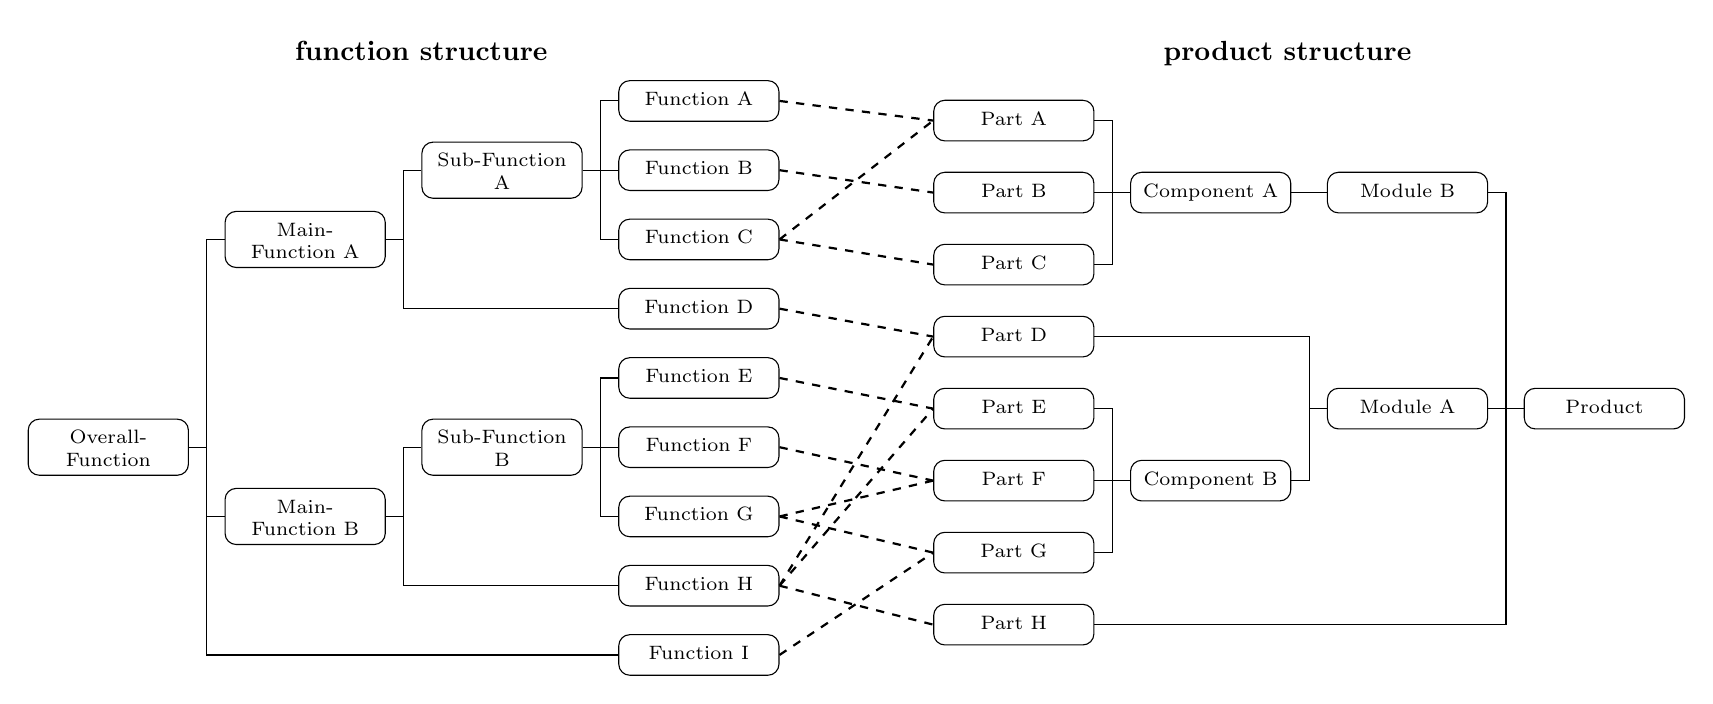
\begin{tikzpicture}
%Define the function structure
\tikzset{
  grow'=right,level distance=25mm, sibling distance =3.5mm,
  execute at begin node=\strut,
  every tree node/.style={
			draw,
			rounded corners,
			anchor = west,
			minimum width=20mm,
			text width=18mm,
			align=center,
			font = {\scriptsize}},
         edge from parent/.style={draw, edge from parent fork right}
}
%Draw the function structure (top to bottom)
%distance from root: width of tree
\begin{scope}[frontier/.style={distance from root=75mm}]
\Tree
[.{Overall-\\ Function}
		[.{Main-\\ Function A}
			[.{Sub-Function\\ A}
			\node(f1){Function A};
			\node(f2){Function B};
			\node(f3){Function C};
			]
			\node(f4){Function D};
		]
		[.{Main-\\ Function B}
			[.{Sub-Function\\ B}
				\node(f5){Function E};
				\node(f6){Function F};
				\node(f7){Function G};
			]
			\node(f8){Function H};
		]
		\node(f9){Function I};
]
\end{scope}
%Define the product structure
\tikzset{grow'=left,
		sibling distance =3.85mm,
       edge from parent/.style={
         draw, edge from parent fork left}
}
%Draw the product structure (bottom up)
%distance from root: width of tree
%xshift/yshift: Shiftoption of right tree
\begin{scope}[
	frontier/.style={distance from root=75mm},
	xshift=190mm,
	yshift=4.9mm]
\Tree
[.{Product}
		\node(p8){Part H};
		[.{Module A}
			[.{Component B}
				\node(p7){Part G};
				\node(p6){Part F};
				\node(p5){Part E};
			]
			\node(p4){{Part D}};
		]
		[.{Module B}
			[.{Component A}
				\node(p3){Part C};
				\node(p2){Part B};
				\node(p1){Part A};
			]
		]
]
\end{scope}
%Draw the lines between function and product side
  \draw [thick, >=stealth, dashed]
        (f1.east)--(p1.west)
        (f2.east)--(p2.west)
        (f3.east)--(p3.west)
        (f3.east)--(p1.west)
        (f4.east)--(p4.west)
        (f5.east)--(p5.west)
        (f6.east)--(p6.west)
        (f7.east)--(p7.west)
        (f7.east)--(p6.west)
        (f8.east)--(p4.west)
        (f8.east)--(p5.west)
        (f8.east)--(p8.west)
        (f9.east)--(p7.west);
%Draw the headlines
\begin{scope}[every node/.style = {rounded corners, font = {\normalsize\bfseries}}]
\node at (5,5) [] {function structure};
\node at (16,5) [rounded corners] {product structure};
\end{scope}
\end{tikzpicture}
\end{document}
